\section{Overview Of Machine Learning Algorithms} \label{sec:ML_BGK}
Machine learning is evolved from a collection of powerful techniques in AI areas. These methods start from training data to learn useful structural patterns and models. A machine learning approach consists of two main phases: the training phase and the decision making phase. In the training phase, after a data mining period that creates a training dataset, machine learning methods are applied to learn a system model. In the decision making phase, the trained model is used to estimate the output corresponding to each new input.
Machine learning algorithms can be distinguished into four main categories: supervised, unsupervised, semi-supervised and reinforcement learning.
\begin{figure}[tb!]
	\centering
	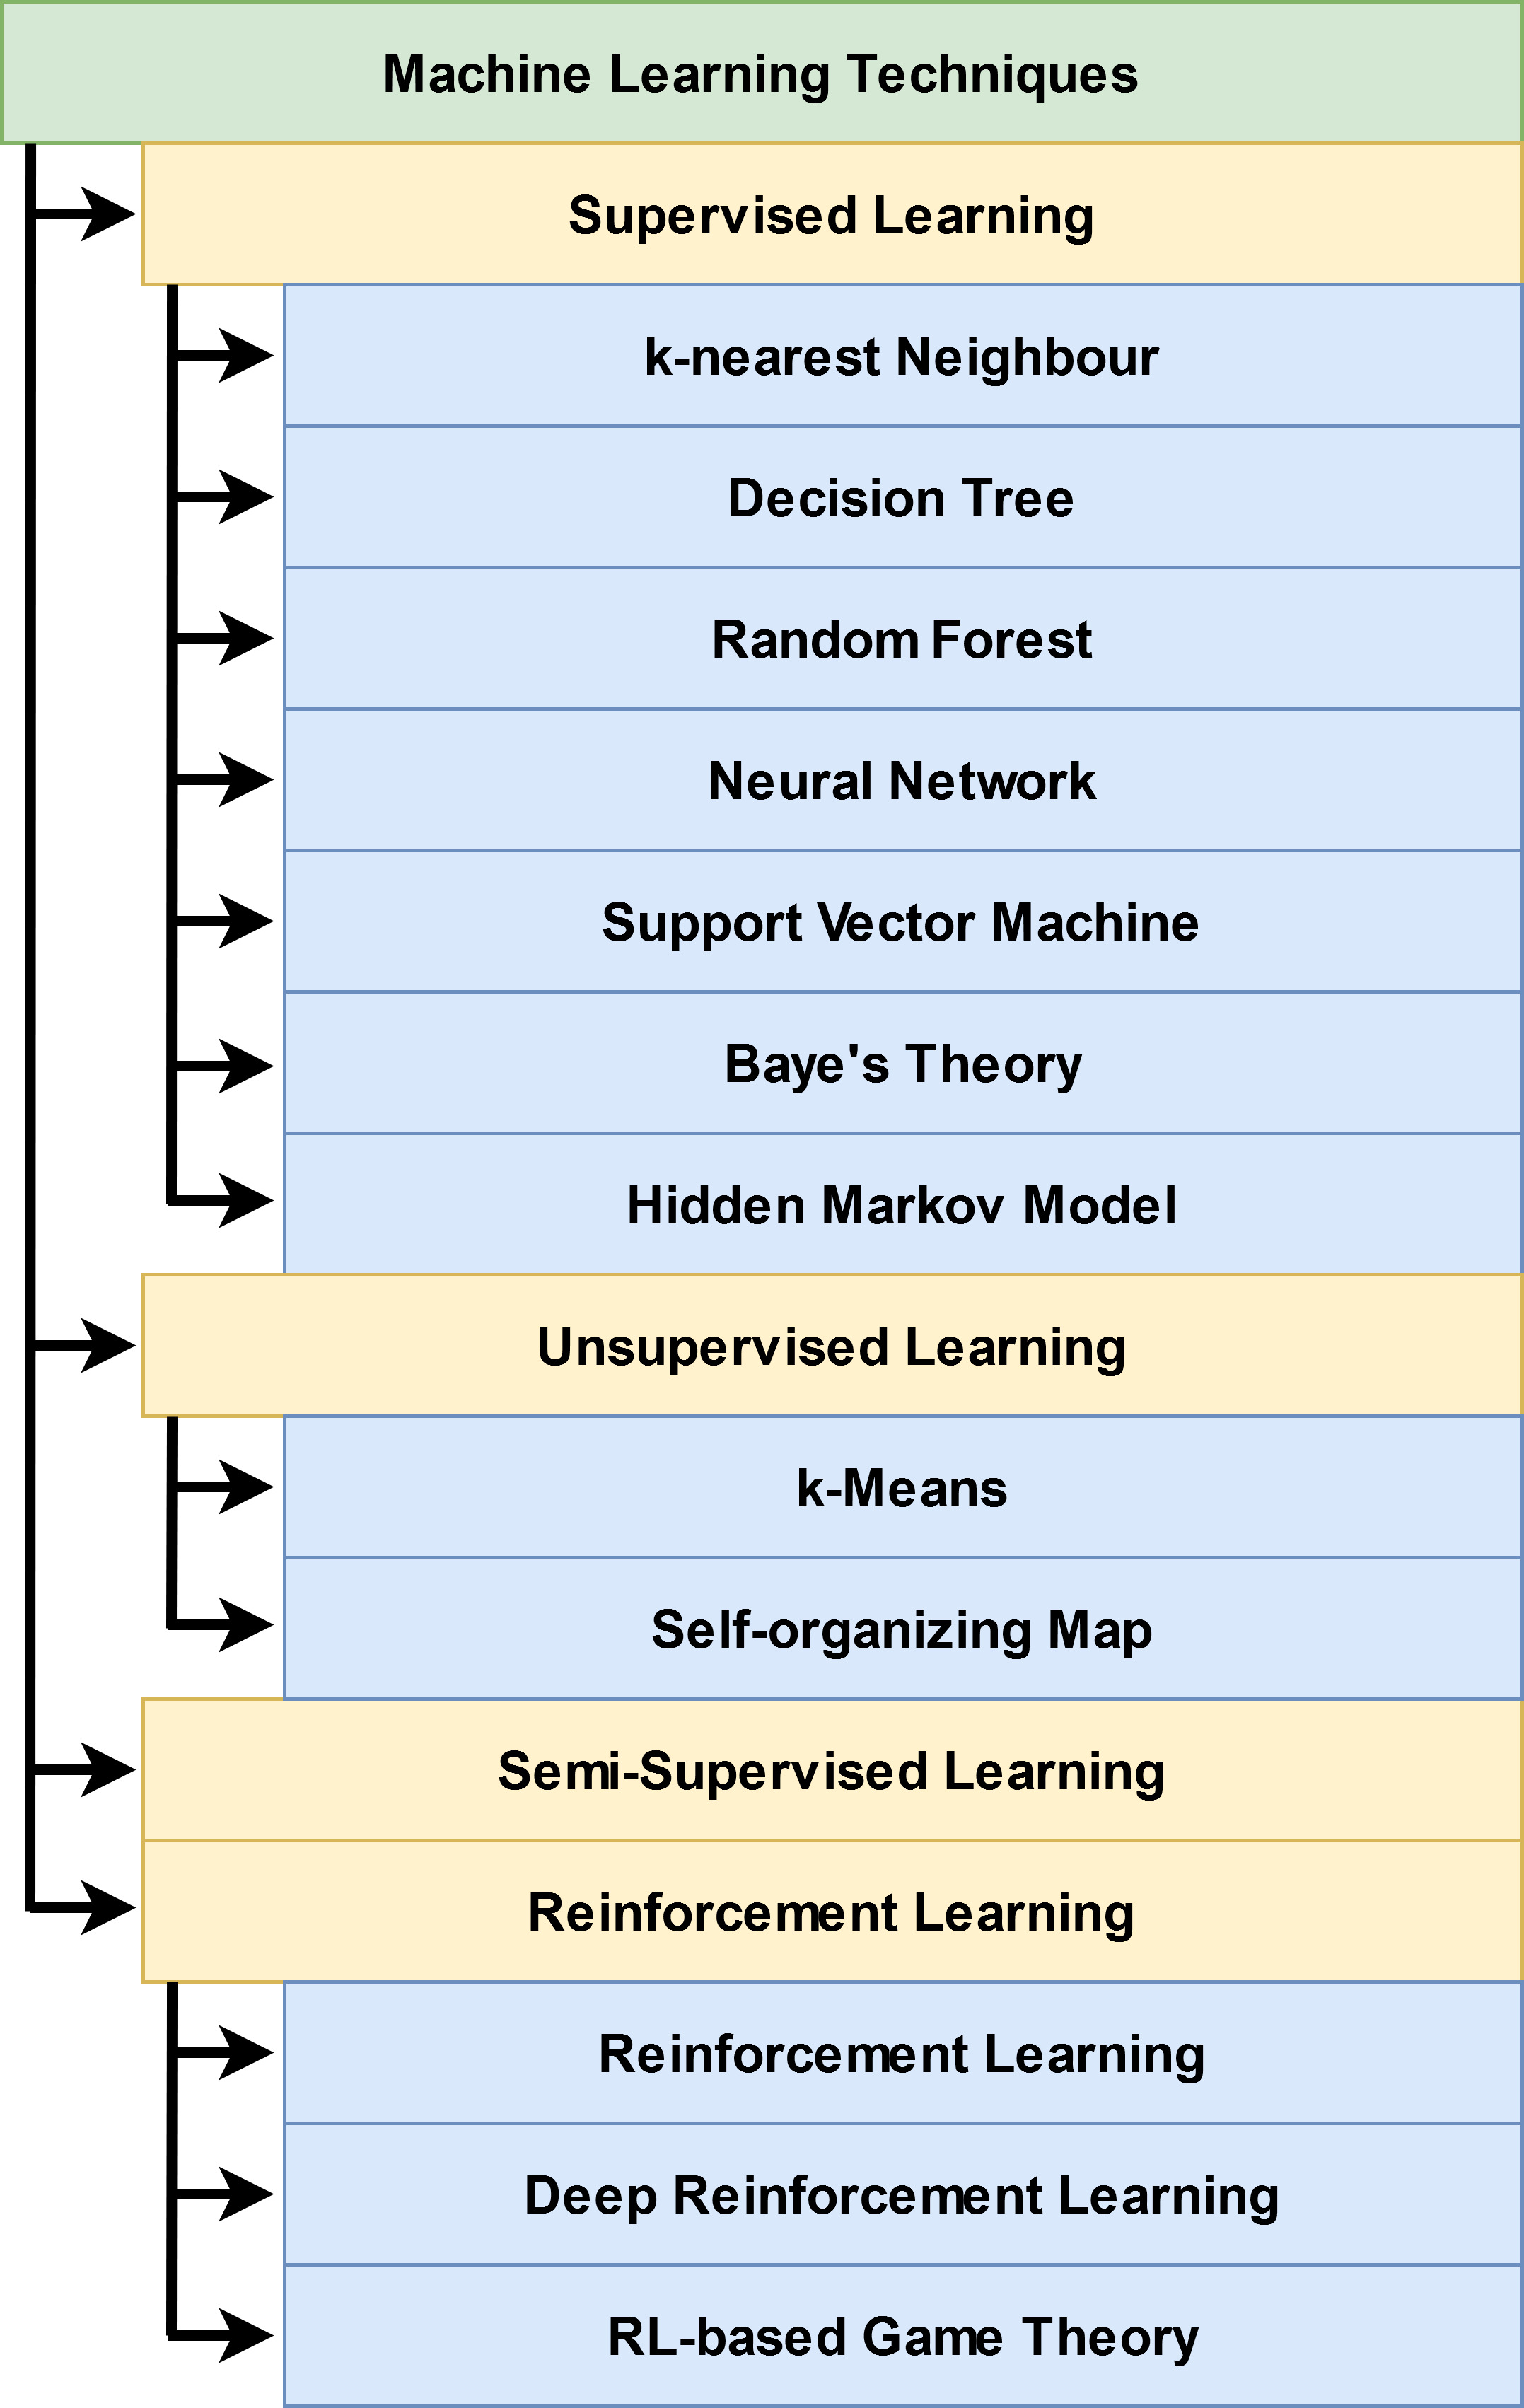
\includegraphics[scale=0.13]{figure/ML_algo.jpg}
	\caption{Common machine learning algorithms.}
	\label{fig:{ML_algo}}
\end{figure}
Each algorithm in Figure \ref{fig:{ML_algo}} is briefly explained with some examples. For a more insightful discussion on machine learning theory, please refer to \cite{Mohammed2016, Marsland2015, Alpaydin2020}.

\subsection{Supervised Learning}
Supervised learning is a kind of labelling learning technique. Supervised learning algorithms are given a labeled training dataset (i.e., inputs and known outputs) to build the system model representing the learned relation between the input and output. After training, when a new input is fed into the system, the trained model can be used to get the expected output \cite{Kotsiantis2007, Hastie2009}. In the following, an exhaustive representation of supervised learning algorithms is provided:
\begin{itemize}
\item[]\textit{1) k-Nearest Neighbor} (k-NN): In k-NN the classification of a data sample is determined based on the k nearest neighbors of that unclassified sample. The process of the k-NN algorithm is very simple: if the most of the k nearest neighbors belong to a certain class, the unclassified sample will be classified into that class. The higher the value of k is, the less effect the noise will have on the classification. Since the distance is the main metric of the k-NN algorithm, several functions can be applied to define the distance between the unlabeled sample and its neighbors, such as Chebyshev, City-block, Euclidean and Euclidean squared \cite{Cover1967}.
\item[]\textit{2) Regresstion Tree}: The RT performs classification through a learning tree. In the tree, each node represents a data feature, all branches represent the conjunctions of features that lead to classifications, and each leaf node is a class label. The unlabeled sample can be classified by comparing its feature values with the nodes of the RT \cite{Han2011}. The RT has many advantages, such as intuitive knowledge expression, simple implementation and high classification accuracy. ID3 \cite{Quinlan1986}, C4.5 \cite{Karatsiolis2012} and CART \cite{Burrows1995} are three widely-used decision tree algorithms. The biggest difference among them is the splitting criteria which are used to build decision trees. 
\item[]\textit{3) Random Forest}: A RF \cite{Breiman1999} consists of many RT. To mitigate over-fitting of RT methods and improve accuracy, the random forest method construct each RT by randomly choosing a subset of the features space . The steps to classify a new data sample by using random forest methods are:
\begin{itemize}
\item[]a) Put the data sample in each tree in the forest;
\item[](b) Each tree gives a classification result (vote);
\item[](c) The data sample will be classified into the class which has more votes.
\end{itemize}
\item[]\textit{4) Neural Network} (NN): A neural network is a computing system composed by a large number of simple processing units, which operate in parallel to learn experiential knowledge from historical data \cite{Haykin}. Each neuron performs highly complex, nonlinear and parallel computations. In a NN, its nodes are the equivalent components of the neurons in the human brain. These nodes use activation functions to perform nonlinear computations. The most frequently used activation functions are the sigmoid and the hyperbolic tangent functions. Simulating the way neurons are connected in the human brain, the nodes in a NN are connected to each other by variable link weights.
A NN has many layers. The first layer is the input layer, the last layer is the output layer and layers between them are the hidden layers. The output of each layer is the input of the next layer and the output of the last layer is the result. By changing the number of hidden layers and the number of nodes in each layer, complex models can be trained to improve the performance of NNs. NNs are widely used in many applications, such as pattern recognition. In figure \ref{fig:{NN_base}} the most basic NN with three layers has been shown. An input has $m$ features (i.e., $X_{1},X_{2},...,X_{m}$) and the input can be assigned to n possible classes (i.e., $Y_{1},Y_{2},...,Y_{n}$). Also, $W_{ij}^{1}$ denotes the variable link weight between the $ith$ neuron of layer $l$ and the $jth$ neuron of layer $l + 1$, and $ak^{l}$ denotes the activation function of the $kth$ neuron in layer $l$.
\begin{figure}[tb!]
	\centering
	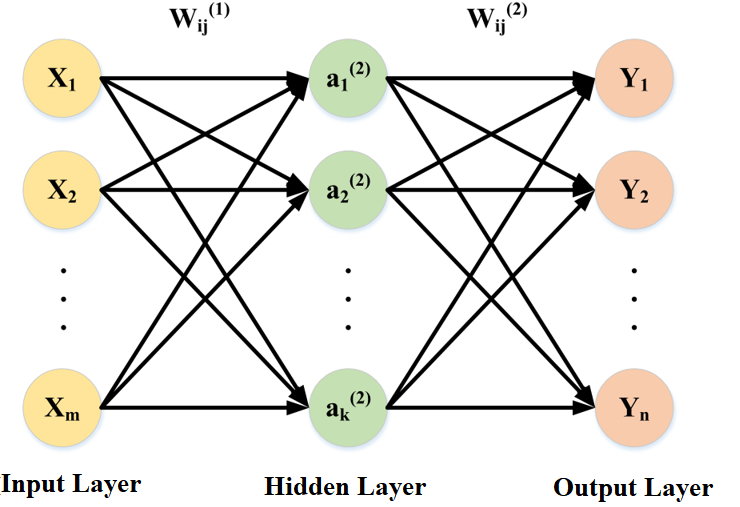
\includegraphics[width=13cm]{figure/NN_base.png}
	\caption{A basic neural network with three layers: an input layer, a hidden layer and an output layer.}
	\label{fig:{NN_base}}
\end{figure}
There are many types of neural networks, which can be divided in supervised or unsupervised main group \cite{Lee2005}. In the following, we will give a brief description of supervised neural networks.
\begin{itemize}
\item[]\textit{a)	Random NN}: The random NN can be represented as an interconnected network of neurons that exchange spiking signals. The main difference between random NN and other neural networks is that neurons in random NN exchange spiking signals probabilistically. In random NN, the internal excitatory state of each neuron is represented by an integer called “potential”. The potential value of each neuron rises when it receives an excitatory spiking signal and drops when it receives an inhibitory spiking signal. Neurons whose potential values are strictly positive are allowed to send out excitatory or inhibitory spiking signals to other neurons according to specific neurondependent spiking rates. When a neuron sends out a spiking signal, its potential value drops one. The random NN has been used in classification and pattern recognition \cite{Timotheou2010}.
\item[]\textit{b)	Deep NN}: Neural networks with a single hidden layer are generally referred to as shallow NNs. In contrast, neural networks with multiple hidden layers between the input layer and the output layer are called deep NNs \cite{LeCun2015, Schmidhuber2015}. To process high-dimensional data and to learn increasingly complex models, deep NNs with more hidden layers and neurons are needed. However, deep NNs increase the training difficulties and require more computing resources. In recent years, the development of hardware data processing capabilities and the evolved activation functions make it possible to train deep NNs \cite{Pandey2014}. In deep NNs, each layer’s neurons train a feature representation based on the previous layer’s output, which is known as feature hierarchy. The feature hierarchy makes deep NNs capable of handling large high-dimensional datasets. Due to the multiple-level feature representation learning, compared to other machine learning techniques, deep NNs generally provide much better performance \cite{Pandey2014}.
\item[]\textit{c)	Convolutional NN}: Convolutional NN and recurrent NN are two major types of deep NNs. Convolutional NN \cite{Krizhevsky2012, Li2018} is a feed-forward neural network. Local sparse connections among successive layers, weight sharing and pooling are three basic ideas of convolutional NN. Weight sharing means that weight parameters of all neurons in the same convolution kernel are same. Local sparse connections and weight sharing can reduce the number of training parameters. Pooling can be used to reduce the feature size while maintaining the invariance of features. The three basic ideas reduce the training difficulties of convolutional NNs greatly.
\item[]\textit{d)	Recurrent NN}: In feed-forward neural networks, the information is transmitted directionally from the input layer to the output layer. However, recurrent NN is a stateful network, which can use internal state (memory) to handle sequential data. Unlike a traditional deep NN, which uses different parameters at each layer, the recurrent NN shares the same parameters across all time steps. This means that at each time step, the recurrent NN performs the same task, just with different inputs. In this way, the total number of parameters needed to be trained is reduced greatly. Long Short-Term Memory (LSTM) \cite{Li2015a} is the most commonly-used type of recurrent NNs, which has a good ability to capture long-term dependencies. LSTM uses three gates (i.e., an input gate, an output gate and a forget gate) to compute the hidden state.
\end{itemize}
\item[]\textit{5) Support Vector Machine} (SVM): SVM is invented by Vapnik and others \cite{Vapnik1999}, which has been widely used in classification and pattern recognition. The basic idea of SVM is to map the input vectors into a high-dimensional feature space. This mapping is achieved by applying different kernel functions, such as linear, polynomial and Radial Based Function (RBF). Kernel function selection is an important task in SVM, which has effect on the classification accuracy. The selection of kernel function depends on the training dataset. The linear kernel function works well if the dataset is linearly separable. If the dataset is not linearly separable, polynomial and RBF are two commonly-used kernel functions. In general, the RBF-based SVM classifier has a relatively better performance than the other two kernel functions.
The objective of SVM is to find a separating hyperplane in the feature space to maximize the margin between different classes. The margin is the distance between the hyperplane and the closest data points of each class. The corresponding closest data points are defined as support vectors.
\item[]\textit{6) Bayes’ Theory}: Bayes’ theory uses the conditional probability to calculate the probability of an event occurring given the prior knowledge of conditions that might be related to the event. The Bayes’ theory is defined mathematically as the following equation:
\begin{equation*}
P(H\vert E)=\dfrac{P(E\vert H)P(H)}{P(E)}
\end{equation*}
where $E$ is a new evidence, $H$ is a hypothesis, $P(H\vert E)$ is the posterior probability that the hypothesis $H$ holds given the new evidence $E$, $P(E\vert H)$ is the posterior probability that of evidence $E$ conditioned on the hypothesis $H$, $P(H)$ is the prior probability of hypothesis $H$, independent of evidence $E$, and $P(E)$ is the probability of evidence $E$.
In a classification problem, the Bayes’ theory learns a probability model by using the training dataset. The evidence $E$ is a data sample, and the hypothesis $H$ is the class to assign for the data sample. The posterior probability $P(H\vert E)$ represents the probability of a data sample belonging to a class. In order to calculate the posterior probability $P(H\vert E)$, $P(H)$, $P(E)$ and $P(E\vert H)$ need to be calculated first based on the training dataset using the probability and statistics theories, which is the learning process of the probability model. When classifying a new input data sample, the probability model can be used to calculate multiple posterior probabilities for different classes. The data sample will be classified into the class with the highest posterior probability $P(H\vert E)$. The advantage of Bayes’ theory is that it requires a relatively small number of training samples dataset to learn the probability model \cite{Box2011}. However, there is an important independence assumption when using the Bayes’ theory. To facilitate the calculation of $P(E\vert H)$, the features of data samples in the training dataset are assumed to be independent of each other \cite{Bakker2017}.
\item[]\textit{7) Hidden Markov Models} (HMM): HMM is one kind of Markov models. Markov models are widely used in randomly dynamic environments which obey the 
memoryless property. The memoryless property of Markov models means that the conditional probability distribution of future states only relates to the value of the current state and is independent of all previous states \cite{Rabiner1989, Holgado2020}. There are other Markov models, such as Markov Chains (MC). The main difference between HMM and other models is that HMM is often applied in environments where system states are partially visible or not visible at all.
\end{itemize}
\subsection{Unsupervised Learning}
In contrast to supervised learning, an unsupervised learning algorithm is given a set of inputs without labels, thus there is no output. An unsupervised learning algorithm aims to find patterns, structures, or knowledge in unlabeled data by clustering sample data into different groups according to the similarity between them. The unsupervised learning techniques are widely used in clustering and data aggregation. In the following, we will give a representation of widely-used unsupervised learning algorithms.
\begin{itemize}
\item[]\textit{1)	k-Means}: The k-means algorithm is used to recognize a set of unlabeled data into different clusters. To implement the kmeans algorithm, only two parameters are needed: the initial dataset and the desired number of clusters. If the desired number of clusters is k, the steps to resolve node clustering problem by using k-means algorithms are:
\begin{itemize}
\item[]\textit{a)} initialize k cluster centroids by randomly choosing k nodes;
\item[]\textit{b)} use a distance function to label each node with the closest centroid;
\item[]\textit{c)} assign new centroids according to the current node memberships;
\item[]\textit{d)} stop the algorithm if the convergence condition is valid, otherwise go back to step \textit{b)}.
\end{itemize}
\item[]\textit{2)	Self-Organizing Map} (SOM): SOM, also known as SelfOrganizing Feature Map (SOFM) \cite{Kohonen2012}, is one of the most popular unsupervised neural network models. SOM is often applied to perform dimensionality reduction and data clustering. In general, SOM has two layers, an input layer and a map layer. When SOM is used to perform data clustering, the number of neurons in the map layer is equal to the desired number of clusters. Each neuron has a weight vector. The steps to resolve data clustering problem by using SOM algorithm are:
\begin{itemize}
\item[]a) initialize the weight vector of each neuron in the map layer;
\item[](b) choose a data sample from the training dataset;
\item[](c) use a distance function to calculate the similarity between the input data sample and all weight vectors. The neuron whose weight vector has the highest similarity is called the Best Matching Unit (BMU). The SOM algorithm is based on competitive learning;
\item[](d) The neighborhood of the BMU is calculated;
\item[](e) The weight vectors of the neurons in the BMU’s neighborhood are adjusted towards the input data sample;
\item[](f) Stop the algorithm if the convergence condition is valid, otherwise go back to step (b).
\end{itemize}
\end{itemize}
\subsection{Semi-Supervised Learning}
Semi-supervised learning is a type of learning which uses both labeled and unlabeled data. Semi-supervised learning is useful due the fact that in many real-world applications, the acquisition of labeled data is expensive and difficults while acquiring a large amount of unlabeled data is relatively easy and cheap. Moreover effective use of unlabeled data during the training process actually tends to improve the performance of the trained model. In order to make the best use of unlabeled data, assumptions have to be hold in semisupervised learning, such as smoothness assumption, cluster assumption, low-density separation assumption, and manifold assumption. Pseudo Labeling \cite{Wu2018} is a simple and efficient semi-supervised learning technique. The main idea of Pseudo Labeling is simple. Firstly, use the labeled data to train a model. Then, use the trained model to predict pseudo labels of the unlabeled data. Finally, combine the labeled data and the newly pseudo-labeled data to train the model again. There are other semi-supervised learning methods, such as Expectation Maximization (EM), co-training, transductive SVM and graph-based methods. Different methods rely on different assumptions. For example, EM builds on cluster assumption, transductive SVM builds on low-density separation assumption, while graph-based methods build on the manifold assumption.
\subsection{Reinforcement Learning}
Supervised learning algorithms are generally applied to conduct classification and regression tasks, while unsupervised and reinforcement learning algorithms are applied to conduct clustering and decision-making tasks respectively.
\begin{itemize}
\item[]\textit{1)	Reinforcement Learning} (RL): RL \cite{Sutton2018, Kaelbling1996} involves an agent, a state space S and an action space A. The agent is a learning entity which interacts with its environment to learn the best action to maximize its long-term reward. The long-term reward is a cumulative discounted reward and relates to both the immediate reward and future rewards. When applying RL to SDN, the controller generally works as an agent and the network is the environment. The controller monitors the network status and learns to make decisions to control data forwarding. Specifically, at each time step $t$, the agent monitors a state $s_{t}$ and chooses an action $a_{t}$ from the action space $A$, receives an immediate reward $r_{t}$ which indicates how good or bad the action is, and transitions to the next state $st+1$. The objective of the agent is to learn the optimal behavior policy $\pi$ which is a direct map from the state space S to the action space $A (\pi : S \longrightarrow A)$ to maximize the expected long-term reward. From the behavior policy $\pi$, the agent can determine the best corresponding action given a particular state. In RL, value function is used to calculate the long-term reward of an action given a state. The most well-known value function is Q-function, which is used by Q-learning to learn a table storing all state-action pairs and their long-term rewards.
\item[]\textit{2)	Deep Reinforcement Learning} (DRL): The main advantage of RL is that it works well without prior knowledge of an exact mathematical model of the environment. However, the traditional RL approach has some shortcomings, such as low convergence rate to the optimal behavior policy $\pi$ and its inability to solve problems with high-dimensional state space and action space. These shortcomings can be addressed by DRL. The key idea of DRL is to approximate the value function by leveraging the powerful function approximation property of deep NNs. After training the deep NNs, given a state-action pair as input, DRL is able to estimate the long-term reward. The estimation result can guide the agent to choose the best action.
\item[]\textit{3)	RL-Based Game Theory}: Game theory is a mathematical tool that focuses on strategic interactions among rational decision-makers. A game generally involves a set of players, a set of strategies and a set of utility functions. Players are decision-makers. Utility functions are used by players to select optimal strategies. In cooperative games, players cooperate and form multiple coalitions. Players choose strategies that maximize the utility of their coalitions. In non-cooperative games, players compete against each other and choose strategies individually to maximize their own utility. In the network field, it is often assumed that nodes are selfish.
In non-cooperative games, players do not communicate with each other, and at the beginning of each play round, players do not have any information about the strategies selected by the other players. At the end of each play round, all players broadcast their selected strategies, which are the only external information. However, each player’s utility can be affected by the other players’ strategies. In this case, adaptive learning methods should be used to predict the strategies of the other players, based on which each player chooses its optimal strategy. RL is a widely-used adaptive learning method, which can help players select their optimal strategies by learning from historical information such as network status, the other players’ strategies and the corresponding utility. Thus, RL-based game theory is an effective decision-making technique.
\end{itemize}

%====================================================================================================
%====================================================================================================
\section{Related Works} \label{RelWorks}
The problems of modeling, managing and optimizing resources in a heterogeneous communication network is a very challenging engineering problem because of its inherent complexity \cite{Neely2010,Lemeshko2019,Tan2017,Abdelmoniem2019}.

Numerous studies have been conducted to maximize the performance of the controller and OpenFlow switch of SDN, however, few results and methodologies exist to model and perform optimal control of SDN switches with priority scheduling. When analyzing the literature regarding traffic management in SDN and priority queueing, we can distinguish three main different approaches.

\textit{Heuristic approaches}, where algorithms to both identify and control traffic within a queue are based on rule-of-thumbs and empirical approaches that do not take into account any particular model: in \cite{Boero2016} a heuristic method is proposed to balance the packet load among queues in order to reduce packet losses, which does not aim at providing an optimal solution; in \cite{Umadevi} authors provide a scheduling algorithm for handling the incoming data traffic by enqueuing packets into the corresponding queue based on priority and High Priority queue is dequeued first; in \cite{Olariu} the authors define multiple queues with different priority classes, which are used to prioritize VoIP packet based on delay, and the controller decides where to enqueue the packet based on delay and considering 5 different decision thresholds.
  
\textit{Parametric approaches}, where the control of queues is based on less heuristics and more objective methods. More precisely, one of more parameters that describe the QoS of an SDN are chosen and optimization is performed based on \textit{static} models characterised by such parameters: both in \cite{Haiyan} and \cite{ChenWang} the authors consider different approaches to model and control queuing delays with specific network parameters; in \cite{Najjar} QoE is taken into account in the context of VOIP and the decision metric for selecting the best link for establishing a new VoIP call is based on the MOS quality metric, which is a typical measure of the level of a user's satisfaction of the quality of a call. These approaches despite the fact that are easy to understand and to implement, may not be often suitable to describe and control traffic flows in large and complex networks as they are not based on a \textit{dynamical} network model.
  
\textit{Model-based approach}, where a \textit{dynamical} mathematical model of packet flows within a queue is considered, is the one most related to the research conducted in this thesis. In the classical literature of queuing theory, in particular applied to SDN, most of the approaches are based on classic structures for models \cite{MDPSDNSURV} and many techinques are exploited to estimate the parameters and the state of a queue \cite{ParameterStateEst}. In \cite{Sood2016PerformanceAO}, the authors emphasized that switch performance depends on multiple factors such as: flow-table size, packet arrival rate, etc., and they took these key factors into account for the design of their M/Geo/1 system where the arriving packets follow a Poisson distribution and the service times follows a Geometric distribution; in \cite{SINGH201824}, beside describing a comprehensive review of the literature (mostly M/M/k and M/G/k), authors derived a new model for a queueing network, based on Quasi Bird Death (QBD) processes; another approach based on a dynamical model for Model Predictive Control is described in \cite{SchoffMPC}, where the authors derive a Discrete Time Markov Jump Linear System to model a queueing network with the aim of defining predictive control policies based on MPC; finally, in \cite{WANG2012120} the author proposes a new congestion control algorithm based on MPC, called MPAQM, where the queue length is predicted based on the extended TCP/AQM system model and a state estimator. The main drawback of the approach proposed by the authors here is that they linearize and discretize the model of a TCP/AQM interconnection system as illustrated in \cite{TCPSTATESPACE}; Nonlinear MPC can be applied, but the problem is that the resulting optimization problem can be nonconvex and so hard to solve. In such scenarios, linearization is a solution but not always a good solution because of the fact that linearize a model of a complex system not always ensure adequate control performance, especially when the system is going to operate far from of the linearization point.
%  
% \textbf{Non ho capito questo ultimo paragrafo: se fanno linearizzazione, perche' si potrebbe usare MPC non lineare? La parte dopo, che dice che con la linearizzazione si possono avere problemi, mi sembra invece giusta. Forse si deve prima dire che la linearizzazione non funziona sempre, e spostare alla fine la frase su nonlinear MPC spiegando pero' che AL POSTO della linearizzazione si puo' direttamente applicare nonlinear MPC, che pero' ha i suoi problemi...giusto?}

Obviously the most interesting are the Model-based approaches. However, their main drawback is related to the identification of the model. One issue is related to the need of having access to the queue's buffer data to identify the model and, at least with commercial hardware, this is not possible in general. A second issue is that classical models, such as the ones previously discussed, are usually designed to provide best accuracy for one step prediction. When applying MPC one wants to forecast and exploit the value of state variables for multiple steps ahead: using classical approaches this is achieved by using the prediction computed at $k+1$ to predict the state at $k+2$, and so on. This approach is not always accurate when a long prediction horizon is considered, since many additional issues arise such as error propagation and increased uncertainty. In such situations, a multiple output strategy where a model is able to directly predict the state at different future time steps, or one model for each time step as we will propose in this work, can increase the MPC performance. Of course this comes with additional computational complexity, especially when the number of time steps to be forecasted increases: however, as will be shown later on, this is not an issue in our methodology since the future predictions can be computed exploiting the advantages of binary decision trees and parallel computation.

The last and most important issue is that the mathematical models proposed in such literature do not allow to directly exploit MPC methods with, simultaneously, good accuracy and a realistically implementable computational complexity, i.e. using Quadratic Programming (QP) solvers. Tackling such research challenges is the main topic of this thesis. Indeed, to the best of the author's knowledge, the state of the art in deriving accurate dynamical models of communication networks still lacks of methods that exploit historical network data to learn (identify) a dynamical network model that can be directly used for optimal control (e.g. of segment routing and/or queue management) and is practical from the computational complexity point of view \cite{Neely2010,Lemeshko2019,Kim2019,Aljoby2019,Lebedenko2018,Le2007,SouravGhosh2005}. This manuscript provides a novel methodology to fill this gap.

In this scenario, computing technologies such as graphic processing and tensor processing units represent a good opportunity to implement advanced control theoretic (e.g. MPC) and machine learning algorithms (e.g. decision trees, deep neural networks, etc.) in the communication networks \cite{Wang2018, Usama2017, Xie2019, Xu2018}. In summary, the real-time programmability of SDN controllers and the availability of massive historical data enable the exploitation of data analysis and optimization techniques for improving networks efficiency and performance.

Other Machine Learning (ML) approaches applied to telecommunication networks has been investigated over the years. A Knowledge Plane (KP) approach \cite{Clark2003} has been proposed to enable automation, recommendation and intelligence by applying ML and cognitive techniques. However the KP approach has not been prototyped nor deployed because each node of traditional network systems, such as routers or switches, can only view and act over a small portion of the system. This implies that each node can learn only from a (small) part of the complete system and therefore it is very complex to design control algorithms beyond the local domain \cite{Mestres2017}. Thanks to SDN the network resources are managed by a logically centralized controller that have a global view of the network \cite{Kreutz2015, Sezer2013, Chen2015, Jarschel2014, Ameigeiras2015}. This feature provides the capacity of collecting data on the network state and opens the possibility of improving the characteristics of each network device with ML algorithms.

Indeed, the most difficult challenge to be addressed in order to apply optimization techniques is to derive a predictive model of the queues of the switch behaviour \cite{Yeremenko2018, John2017, Yang2011, Bahnasy2018, Zhang2014}. On this line of research, Cello \textit{et al.} provide in \cite{Cello2016} a predictive model for estimating QoS in order to detect the need for a re-routing strategy due to link saturation. However, this framework cannot be used to apply traffic optimization techniques. In \cite{LeeIEEEToN2007} an initial effort is conducted to derive a general hybrid systems framework to model the flow of traffic in communication networks. In \cite{DiBenedetto2014} the authors provide a first formulation and implementation, based on hybrid systems theory, of a mathematical and simulative environment to formally model the effect of router/link failures on the dynamics of TCP and UDP packet flows belonging to different end-user services (i.e. http, ftp, mailing and video streaming). However, even though hybrid systems are very effective in modelling a network of routers, using such framework for implementing traffic optimization is out of question for computational complexity issues. A further research question focuses on designing strategies for periodic updating of network models, in order to maintain good performance despite the evolution of the real system \cite{Mulinka2018}.

Deriving accurate dynamical models of communication networks that can be directly used for optimal control by the exploitation of historical network data is still a challenging and actual problem \cite{Kim2019,Aljoby2019,Lebedenko2018,Le2007,SouravGhosh2005}.

Recent advances in computing technologies such as Graphics Processing Unit and Tensor Processing Unit provide a good opportunity to apply promising machine learning techniques (e.g., deep neural networks) in the network field \cite{Wang2018, Usama2017}. Data is the key to the data-driven machine learning algorithm: the centralized SDN controller has a global network view, and is able to collect various network data. The potential impact of machine learning in networks is evident from the huge literature on the topic: Patcha and Park \cite{Patcha2007} have given a detailed description of machine learning techniques in the domain of intrusion detection; Nguyen and Armitage \cite{Nguyen2008} focus on IP traffic classification; Bkassiny et al. \cite{Bkassiny2013} have surveyed existing machine learning based methods in Cognitive Radio Networks; \cite{Alsheikh2014} investigated how machine learning techniques can be applied in wireless sensor networks; Wang et al. \cite{Wang2015} have presented the state-of-the-art on Artificial Intelligence based techniques applied to evolve heterogeneous networks and discussed future research challenges; Buczak and Guven \cite{Buczak2016} investigated data mining methods for cyber-security intrusion detection; Klaine et al. \cite{Klaine2017} have surveyed machine learning algorithms for self organizing cellular networks; \cite{Fadlullah2017} investigated how to improve network traffic control using machine learning techniques; Hodo et al. \cite{Hodo2017} focus on machine learning based Intrusion Detection System; Zhou et al. \cite{Zhou2017} focus on cognitive radio technologies enforced by machine learning techniques to enhance spectrum utilization and energy efficiency of wireless networks; Chen et al. \cite{Chen2017} have studied neural networks solutions applied in wireless networks for virtual reality and edge caching; Usama et al. \cite{Usama2017} have applied unsupervised learning techniques in the general domain of networking. Although machine learning techniques have been widely investigated in the communication scientific community, to the best of our knowledge no existing work focuses on the applications of machine learning and control theory for identifying models of network devices in the domain of Software Defined Network (SDN), with the aim of efficiently apply Model Predictive Control.